\section{Introduction}
Proton exchange membrane fuel cells (PEMFCs), henceforth denoted as fuel cells, facilitate the direct conversion of chemical energy present in hydrogen into electrical energy.
% 质子交换膜燃料电池(PEMFC),以下称为燃料电池,有助于将氢气中的化学能直接转化为电能。
These fuel cells are characterized by their high energy utilization rate, low operating temperature, and the production of water as the sole reaction byproduct.
% 这些燃料电池的特点是能量利用率高、工作温度低以及产生水作为唯一的反应副产物。
Their versatility allows them to function not only as a small-scale distributed power supply but also as the energy source for high-power transportation systems, thus demonstrating their broad applicability \cite{sharafOverviewFuelCell2014} .
% 它们的多功能性使它们不仅可以作为小型分布式电源,还可以作为大功率运输系统的能源,从而展示了其广泛的适用性\cite{sharafOverviewFuelCell2014}。
Nevertheless, the reliability, stability, and durability of the fuel cell stack, as the central component of the fuel cell power system, have emerged as critical factors influencing the extensive commercialization of fuel cell products.
% 然而,燃料电池电堆作为燃料电池动力系统的核心部件,其可靠性、稳定性和耐用性已成为影响燃料电池产品广泛商业化的关键因素。
% TODO: 尽可能去掉精确的数字表达。讲 水很重要,干燥会造成什么样的影响。缺水会导致什么样的损伤。
% TODO: 浓缩含水检测的方法
% TODO: 把含水状态检测方法的部分分别讲一下优缺点
% TODO: 基于阻抗的和基于含水量的方法之间有什么区别
During the operational phase of the fuel cell, it is imperative to maintain the internal proton exchange membrane (PEM) in an optimal state of hydration to ensure the proton conduction ability remains at its peak, thereby achieving efficient and stable output performance of the fuel cell. Hydration state failure is the most prevalent failure mode of fuel cells, accounting for approximately 52 of total failures, primarily manifested as drying and flooding. Short-term hydration state failure can induce fluctuations and reductions in the output performance of the fuel cell. If this condition persists, it may lead to irreversible attenuation.
% 在燃料电池运行阶段,必须保持内部质子交换膜(PEM)处于最佳水合状态,以保证质子传导能力保持在峰值,从而实现燃料电池高效稳定的输出性能。水合状态失效是燃料电池最常见的失效模式,约占总失效的 52 例,主要表现为干燥和水淹。短期水合状态失效会引起燃料电池输出性能的波动和降低。如果这种情况持续存在,可能会导致不可逆的衰减。
\par
Under dry failure, the water content inside the stack is too low to keep an sufficiently hydrated state,
and the internal resistance increases and heat production increases since some region of the PEM are not fully hydrated.
Long-term dryness may even cause mechanical damage to the PEM, resulting in irreversible damage\cite{pattersonDamageCathodeCatalyst2006}.
% 在干燥失效的情况下,电堆内部的含水量太低,无法保持足够的水合状态,由于质子交换膜的某些区域没有完全水合,内阻增加,产热量增加。长期干燥甚至可能对质子交换膜造成机械损伤,造成不可逆的损坏\cite{pattersonDamageCathodeCatalyst2006}。
Under flooding failure, the water content inside the stack is too high, and the liquid water gradually block the flow channel or reaction area,preventing the reaction gas from reaching the reaction site, causing a local "starvation" phenomenon\cite{chuExperimentalStudyInfluence2022,ohsModelingHydrogenStarvation2011}.
% 在淹没失效情况下,电堆内部含水量过高,液态水逐渐堵塞流道或反应区域,阻止反应气体到达反应现场,造成局部“饥饿”现象
In severe cases, other side reactions  will occur in the fuel cell at this time, causing damage to the carbon carrier\cite{ohsModelingHydrogenStarvation2011,kuracinaStudySelectedCharacteristics2014,jiaMitigationStrategiesHydrogen2017}.
% 严重的情况下,此时燃料电池中会发生其他副反应,对碳载体造成损害
\par
In addition to the direct impact on output performance, the internal hydration state also indirectly affects environmental adaptability and durability\cite{yuanModelbasedObserversInternal2020,fuFuelCellHumidity2021}. In low temperature conditions, especially in sub-zero environments, the free water inside the fuel cell will freeze, thereby blocking the reactant channels, and even causing structural damage to the catalyst layer and diffusion layer\cite{taccaniEffectFlowField2011,doddsHydrogenFuelCell2015}. In addition, it will also affect the aging characteristics of the catalyst\cite{pattersonDamageCathodeCatalyst2006,sunModelingInfluenceGDL2005}. Flooding conditions will accelerate the loss of Pt surface area, while dry conditions will accelerate the corrosion of the carbon carrier \cite{yousfisteinerDiagnosisPolymerElectrolyte2011,chenOperationCharacteristicsCarbon2015}.
% 除了直接影响输出性能外,内部水合状态还间接影响环境适应性和耐久性。在低温条件下,尤其是零度以下的环境下,燃料电池内部的游离水会结冰,从而堵塞反应物通道,甚至造成催化剂层和扩散层的结构损坏。此外,它还会影响催化剂的老化特性。水淹条件会加速 Pt 表面积的损失,而干燥条件会加速碳载体的腐蚀。
\par
Currently, studies focusing on the characterization of the internal hydration state of fuel cells have yielded significant findings. Standard indicators utilized for ascertaining the hydration state of fuel cells encompass direct observation or computation of water content, electrical signals, pressure drop signals, and electrochemical signals \cite{hussainiVisualizationQuantificationCathode2009}.
% 目前,针对燃料电池内部水合状态表征的研究已经取得了重要的发现。用于确定燃料电池水合状态的标准指标包括直接观察或计算水含量、电信号、压降信号和电化学信号
\par
The identification of a fuel cell's hydration state fundamentally involves determining the internal water content, making this the most basic and accurate assessment. Direct observation of water content can be facilitated through the transparent cell method and the neutron imaging method. The transparent cell method modifies the traditional fuel cell structure, employing transparent end plates and flow field plates to directly observe the quantity of liquid water within the flow field\cite{leeVisualizationFloodingSingle2012}. Hussaini et al\cite{hussainiVisualizationQuantificationCathode2009} designed a fuel cell with an effective area of 14cm², containing seven straight channels, and conducted a visual examination of the liquid water content in the fuel cell channels under typical automotive conditions. Yang et al\cite{yangVisualizationLiquidWater2004} utilized a transparent fuel cell for experiments to observe the process of liquid water transfer, discovering that water droplets initially appear on the GDL surface and adhere to the GDL surface due to surface tension. The water droplets progressively enlarge until they make contact with the flow channel wall, which exhibits stronger hydrophilicity. If the droplets on the flow channel are sufficiently thick, they may obstruct the channel and disrupt the airflow. The neutron imaging method is predicated on the principle that rays will attenuate when traversing an object. Given that different materials exhibit varying attenuation characteristics for neutron beams, particularly as water has higher absorbency than other materials such as metals, the internal water content can be measured using the transmitted neutron dose rate. Pekula\cite{pekulaStudyWaterDistribution2005} and Trabold\cite{traboldSituInvestigationWater2006} employed neutron imaging technology and found that water accumulation is likely to occur where the flow channel turns, providing appropriate explanations for each. However, the high cost and complex operation of current neutron imaging equipment have limited its widespread adoption.
% 燃料电池水合状态的识别从根本上涉及确定内部含水量,这是最基本、最准确的评估。通过透明池法和中子成像法可以方便地直接观察水分含量。透明电池方法修改了传统燃料电池结构,采用透明端板和流场板直接观察流场内液态水的量\cite{leeVisualizationFloodingSingle2012}。Hussaini 等人\cite{hussainiVisualizationQuantificationCathode2009}设计了一个有效面积为 14cm²的燃料电池,包含七个直通道,并在典型的汽车条件下对燃料电池通道中的液态水含量进行了目视检查。Yang 等人\cite{yangVisualizationLiquidWater2004}利用透明燃料电池进行实验,观察液态水转移的过程,发现水滴最初出现在 GDL 表面上,并由于表面张力而粘附在 GDL 表面上。水滴逐渐增大直至与流道壁接触,表现出更强的亲水性。如果流道上的液滴足够厚,它们可能会阻塞通道并扰乱气流。中子成像方法基于射线穿过物体时会衰减的原理。鉴于不同的材料对中子束表现出不同的衰减特性,特别是当水比金属等其他材料具有更高的吸收性时,可以使用透射中子剂量率来测量内部含水量。Pekula\cite{pekulaStudyWaterDistribution2005}和 Trabold\cite{traboldSituInvestigationWater2006}采用中子成像技术,发现水流通道转弯处很可能发生积水,并为两者提供了适当的解释。然而,当前中子成像设备的高成本和复杂的操作限制了其广泛采用。
\par
Consequently, researchers have considered utilizing the law of conservation of mass to compute the water content within the fuel cell. When the fuel cell is operating stably, the flow rate of residual water can be calculated by measuring the discharged water. Zhao et al\cite{zhaoStudyWaterTransport2021} employed a single transparent fuel cell with an active area of 25cm to conduct tests under varying operating conditions.
% 因此,研究人员考虑利用质量守恒定律来计算燃料电池内的水含量。当燃料电池稳定运行时,通过测量排出的水量即可计算出残留水的流量。赵等人\cite{zhaoStudyWaterTransport2021}采用活性面积为 25cm 的单个透明燃料电池在不同的操作条件下进行测试。
By comparing the calculated rate of change in water content within the fuel cell and the water distribution in the flow channel, the accuracy of the model was validated.
% 通过比较计算出的燃料电池内含水量的变化率和流道内的水分布情况,验证了模型的准确性。
\par
The output voltage of the fuel cell serves as the most direct indicator of judgment, and faults in the internal hydration state will directly influence the output voltage, causing it to decrease or fluctuate. Particularly for high-power fuel cell systems, the Cell Voltage Monitoring module (CVM) is often the simplest standard of judgment. In terms of the impact of hydration state faults on voltage, recognition standards based on electrical signals encompass polarization curves and voltage fluctuation signals.
% 燃料电池的输出电压是最直接的判断指标,内部水合状态出现故障会直接影响输出电压,导致输出电压降低或波动。特别是对于大功率燃料电池系统,电池电压监测模块(CVM)往往是最简单的判断标准。对于水化状态故障对电压的影响,基于电信号的识别标准包括极化曲线和电压波动信号。
\par
Li et al.\cite{liReviewWaterFlooding2008} showed that at low current densities, water flooding have little effect on the polarization curve. As the current density increases, the voltage drop gradually becomes apparent. The more severe the water flooding, the more severe the voltage decay, and the earlier occurrence of voltage decay. Legros et al\cite{legrosFirstResultsPEMFC2011} introduced dry and wet gases into a single cell, respectively, and found that the fluctuation of the output voltage increased with the current density during dry periods.
% Li 等人\cite{liReviewWaterFlooding2008}表明,在低电流密度下,注水对极化曲线影响很小。随着电流密度的增加,电压降逐渐变得明显。水淹越严重,电压衰减越严重,并且电压衰减发生得越早。Legros 等人\cite{legrosFirstResultsPEMFC2011}分别将干燥和潮湿的气体引入单个电池中,发现在干燥期间输出电压的波动随着电流密度的增加而增加。
\par
The pressure drop between the inlet and outlet of the fuel cell is mainly caused by the friction between the flowing medium and the internal flow channel of the cel\cite{wuDiagnosticToolsPEM2008}. The pressure drop between the two ends increases with the increase of liquid water content, so the pressure drop can well reflect the degree of water flooding in the stack. The indicators include: pressure drop, pressure drop residual, pressure drop frequency, two-phase flow Multiplier coefficient, etc., and the, diagnosis is carried out through the above indicators by qualitative analysis, statistical analysis, artificial intelligence analysis, etc.\cite{liNovelApproachDetermine2017}
% 燃料电池入口和出口之间的压降主要是由流动介质与 cel\cite{wuDiagnosticToolsPEM2008}内部流道之间的摩擦引起的。两端之间的压降随着液态水含量的增加而增大,因此压降可以很好地反映烟囱内水淹的程度。指标包括:压降、压降残余、压降频率、两相流乘数系数等,通过定性分析、统计分析、人工智能分析等,通过上述指标进行诊断。引用{liNovelApproachDetermine2017}
\par
\begin{figure}[h]
	\centering

	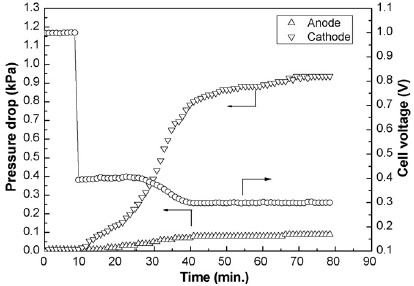
\includegraphics{Research_pictures/Fig1.jpg}
	% \includesvg{Research_pictures/1.svg}
	% \includegraphics{Research_pictures/1.svg}
	\caption[short]{The change of cathode and anode voltage drop with time during flooding process}
	\label{fig:figure1}
\end{figure}
The detection methods based on electrochemical signals mainly include electrochemical impedance spectroscopy, current interruption method, and cyclic voltammetry, etc. Among them, electrochemical impedance spectroscopy is the most common hydration state detection method because it can distinguish different electrochemical processes and can be tested online \cite{yousfisteinerDiagnosisPolymerElectrolyte2011,chenOperationCharacteristicsCarbon2015}. The figure \ref{fig:figure1} shows the difference in fuel cell impedance spectra under different air humidity conditions. As the air humidity decreases, the value of the high-frequency impedance segment (i.e., the intercept of the impedance spectrum with the real axis) gradually increases, the impedance spectrum moves to the right, and the radius of the low-frequency arc segment also gradually increases \cite{hussainiVisualizationQuantificationCathode2009}, which can be used as an indicator of the hydration state of the fuel cell.
% 基于电化学信号的检测方法主要有电化学阻抗谱、电流中断法、循环伏安法等。其中,电化学阻抗谱是最常见的水化状态检测方法,因为它可以区分不同的电化学过程,并且可以在线测试\ 引用{yousfisteinerDiagnosisPolymerElectrolyte2011,chenOperationCharacteristicsCarbon2015}。图\ref{fig:figure1}显示了不同空气湿度条件下燃料电池阻抗谱的差异。随着空气湿度的降低,高频阻抗段的值(即阻抗谱与实轴的截距)逐渐增大,阻抗谱向右移动,低频圆弧段的半径增大 也逐渐增加\cite{hussainiVisualizationQuantificationCathode2009},可以作为燃料电池水合状态的指标。
\par
When analyzing the relationship between impedance spectra and the internal hydration state of fuel cells, equivalent circuit models are often introduced. The model generally includes resistors, capacitors, inductors, and Warburg elements\cite{tangRecentProgressUse2020}. The model is capable of quantitatively analyzing the electrochemical process.  The key to this method is the establishment of equivalent models and parameter identification. Fouquet et al.[25] extended the standard capacitor to a constant phase element, proving that the three resistance values of the model are related to the relative humidity of the air supply. Zhang et al.[26] used a neural network method to complete parameter identification, and the predicted Nyquist plot almost completely coincides with the measured value, and by directly predicting the parameters of the equivalent circuit, they detailed the degree of influence of different processes on fuel cell performance. BMW proposed a method for online monitoring of impedance, which requires collecting five frequency points, divided into three groups to fit the Randles circuit, obtaining ohmic impedance, polarization resistance and double layer capacitance\cite{fouquetModelBasedPEM2006}.
% 在分析阻抗谱与燃料电池内部水合状态之间的关系时,常常引入等效电路模型。该模型通常包括电阻器、电容器、电感器和 Warburg 元件\cite{tangRecentProgressUse2020}。该模型能够定量分析电化学过程。该方法的关键是等效模型的建立和参数辨识。Fouquet 等人 [25] 将标准电容器扩展为恒相位元件,证明模型的三个电阻值与送风相对湿度有关。张等 [26] 他们利用神经网络方法完成参数辨识,预测的奈奎斯特图与测量值几乎完全吻合,并通过直接预测等效电路的参数,详细说明了不同工艺对燃料电池性能的影响程度。BMW 提出了一种在线监测阻抗的方法,需要采集 5 个频点,分成 3 组来拟合 Randles 电路,得到欧姆阻抗、极化电阻和双层电容\cite{fouquetModelBasedPEM2006}。
\par
However, the above methods are mostly suitable for single cells or low-power fuel cells. Applying them to high-power fuel cell doesn't gain any noticeable improvements\cite{tangRecentProgressUse2020,jiangMicrobialFuelCell2018,dotelliCombiningElectricalPressure2016,millerReviewPolymerElectrolyte2011,nagulapatiMachineLearningBased2023}, since the assembly structure, flow field structure, and operating conditions of high-power fuel cell stacks are significantly different from those of single cells and low-power stacks \cite{verhaertWaterManagementAlkaline2011}.
% 然而,上述方法大多适用于单电池或小功率燃料电池。将它们应用于高功率燃料电池并没有获得任何明显的改进\cite{tangRecentProgressUse2020, JiangMicrobialFuelCell2018,dotelliCombiningElectricalPressure2016,,nagulapatiMachineLearningBased2023},因为高功率燃料电池堆的装配结构、流场结构和运行条件显着 与单电池和低功率电堆不同。因此,大功率燃料电池系统水合状态的检测还处于比较空白阶段。
\par
Furthermore, research has indicated that smaller-scale fuel cell stacks exhibit reduced sensitivity to gas flow rates\cite{bonnetDesign80kWePEM2008}, which can also cause the difference between small and big stacks.
% 小尺寸电堆对于气体流量更不敏感

% TODO 这里需要添加一些参考文献
Therefore, the detection of the hydration state of high-power fuel cell systems is still in a relatively blank stage.


\par
Additionally, the variation in the number of cells within a fuel cell stack can significantly influence the power generation performance, leading to temperature imbalances\cite{millerReviewPolymerElectrolyte2011}. This, in turn, further exacerbates the uneven distribution of water present throughout the stack. Consequently, there exists a pronounced distinction between smaller and larger stacks regarding these phenomena.
% 电堆中 Cell 数量的多寡会影响性能,也会导致温度不均衡,进而导致水存量的不均衡
Researches indicates that there may exist notable differences in the water generation mechanisms between large-scale and small-scale polymer electrolyte membrane fuel cell (PEMFC) stacks\cite{jiReviewWaterManagement2009}. Therefore, traditional approaches relying on electrochemical analysis and similar techniques may not be applicable to large-scale stacks. Due to the fact that large-scale fuel cell stacks frequently operate at lower power densities\cite{shojayianSimulationCathodeCatalyst2024}, this could potentially have an impact on the water generation mechanisms involved, further differentiating them from their smaller-scale counterparts.
% 解释了 PEMFC 中水管理问题,提及了大型电堆可能与小型电堆的水生成机理有区别

% 大型电堆通常在低功率密度下工作,这可能会对水生成带来一定的影响 [4]
\par
Consequently, this study aims to investigate the hydration state of high-power fuel cell systems, construct, and validate a water balance model. Initially, the water balance model of the high-power fuel cell system is scrutinized, and a condensation-type exhaust water collection device is established to compute the water flow rate emanating from the fuel cell system.
To authenticate the constructed water balance model, controlled variable experiments are executed under varying working temperatures, air metering ratios, and load currents. The experimental outcomes indicate that as the working temperature and air metering ratio escalate, the water flow rate emanating from the air side incrementally increases, and the water flow rate from the hydrogen side gradually diminishes.
As the load current amplifies, the water flow rate emanating from both sides augments. Ultimately, predicated on the experimental data, the change rate of the internal water content of the fuel cell system under diverse conditions is calculated. The results reveal that under the same load current, as the working temperature and the air stoichiometric ratio augment, the change rate of the internal water content of the fuel cell system progressively decreases.
Conversely, as the load current intensifies, the impact of the air stoichiometric ratio also incrementally escalates. Therefore, at low power, it is essential to maintain an appropriate working temperature, while at high power, upholding an appropriate metering ratio is of greater significance.

% 因此,本研究旨在研究高功率燃料电池系统的水合状态,构建并验证水平衡模型。首先,仔细研究了大功率燃料电池系统的水平衡模型,并建立了冷凝式废水收集装置来计算从燃料电池系统排出的水流量。为了验证所构建的水平衡模型,在不同的工作温度、空气计量比和负载电流下进行了受控变量实验。实验结果表明,随着工作温度和空气计量比的升高,空气侧出水流量逐渐增大,氢气侧出水流量逐渐减小。随着负载电流的增大,从两侧流出的水流量增大。最终根据实验数据计算出不同条件下燃料电池系统内部含水量的变化率。结果表明,在相同负载电流下,随着工作温度和空气化学计量比的增大,燃料电池系统内部含水量的变化率逐渐减小。相反,随着负载电流的增强,空气化学计量比的影响也逐渐增大。因此,在低功率时,保持适当的工作温度至关重要,而在高功率时,保持适当的计量比则更为重要。
\par
Based on the experiment results, we propose the following viewpoint: The water generation and water balance models for large-scale fuel cell stacks differ mechanistically from those of smaller-scale models and cannot be considered as linear scalings of the smaller models. The internal states of large-scale fuel cell stacks exceed the complexity of small-scale stacks due to their increased scale. Consequently, traditional approaches based on small-scale stacks may not be entirely applicable to large-scale stacks.
